\documentclass[a5paper,
              twoside,
              headings=small,
              titlepage=firstiscover,
              numbers=noenddot]{scrbook}

\usepackage[sjannon] {ofs}\OFSfamilydefault [JannonTModerne]

\usepackage{ucs} 						
\usepackage[czech]{babel}
\usepackage[utf8]{inputenc}
\usepackage[T1]{fontenc}

\usepackage{graphicx}
\usepackage{url}

\usepackage{tikz}
\usetikzlibrary{shadows}

\setcounter{figure}{0}
\renewcommand{\thefigure}{\arabic{figure}}

\newcommand*\keystroke[1]{%
  \tikz[baseline=(key.base)]
    \node[%
      draw,
      fill=white,
      drop shadow={shadow xshift=0.25ex,shadow yshift=-0.25ex,fill=black,opacity=0.75},
      rectangle,
      rounded corners=2pt,
      inner sep=1pt,
      line width=0.5pt,
      font=\scriptsize\sffamily
    ](key) {#1\strut}
  ;
}


\begin{document}

\title{Začínáme s~Fedorou}
\subtitle{seznámení s~operačním systémem a první kroky v~systému}
\date{}
\maketitle

\cleardoublepage

\chapter*{Úvod}
Rozhodli jste se, že na svou pracovní stanici, desktop, notebook, netbook\dots (říkejme tomu prostě počítač) nainstalujete jako operační systém právě Fedoru (tzv. linuxovou distribuci). Jak dál? V~čem jsou její největší výhody oproti jiným operačním systémům? Jak se k~Fedoře dostat a jak ji nainstalovat? Jak si Fedoru vylepšit k~obrazu svému a přizpůsobit ji pro konkrétní účel? Pojďme se na to krok za krokem podívat.

\chapter*{O~čem je Fedora}
\section*{Pro koho je?}
Fedora v~edici \emph{Workstation} cílí na uživatele, jejichž primárním zájmem je tvůrčí práce, ať už se jedná o~vývoj nebo jiné činnosti. Nabízí odladěné prostředí \emph{GNOME~3} a spektrum aplikací jako jsou pro vývojáře nástroje \emph{DevAssistant} nebo nově \emph{Builder}, různé aplikace pro virtualizaci (\emph{Boxes}), správu kontejnerů (\emph{Docker}) a dalších. Znamená to, že Fedora rezignuje na běžného uživatele a opouští ho? Ne, Fedoru lze stejně tak dobře použít i pro multimediální účely, mezi které můžeme počítat i střih videa (\emph{PiTiVi}), nebo práci s~bitmapovou (\emph{GIMP}) a vektorovou (\emph{Inkscape}) grafikou. V~určitém smyslu je tak Fedora lepším operačním systémem i pro běžného uživatele, než byla kdy dříve.  

\section*{Otevřenost}
Fedora je linuxový operační systém s~desetiletou tradicí vyvíjený komunitou, tedy profesionálními vývojáři a dobrovolníky bez rozdílu. Vždy obsahovala a bude obsahovat jen svobodný, čili takový software, který je open source a může být volně šířen, upravován a používán za libovolným účelem. Fedora neobsahuje software, na který byste si nemohli \uv{sáhnout} na úrovni zdrojového kódu. Zároveň ale nijak neomezuje software, který si do systému nainstalujete. Ať již jako jednotlivý balík nebo formou repozitáře (zdroje software, viz kapitola {\it Instalace nového software}) %zde muze byt odkaz
třetí strany. Chcete \emph{Google Chrome}? Budete ho mít. Ale i bez toho naleznete v~repozitářích Fedory takřka dvacet tisíc balíků obsahujících nejrůznější aplikace a knihovny. Není to ale jen o~licenční čistotě. Fedora důsledně ctí patentové právo v~oblasti software (jakkoliv je v~rámci EU méně relevantní). Při nasazení Fedory v~komerčním i jiném prostředí máte jistotu, že jednáte v~souladu se zákonem.

\section*{Bezpečnost a soukromí}
Vývoj Fedory má svá jasná pravidla a bezpečnost je priorita. Ve Fedoře probíhá testování jako u~kteréhokoli jiného významného softwarového produktu. Navíc se Fedora každých několik let stává základem, na kterém staví firma Red Hat svůj linuxový operační systém s~komerční podporou -- Red~Hat Enter\-prise Linux~(RHEL). Stejná firma také platí mnoho vývojářů zapojených do projektu Fedory a vlastní ochranné známky s~Fedorou související. Podpora Fedory, která se počítá od data vydání aktuální verze systému po vydání verze další plus jeden měsíc (což při dodržení šestiměsíčního cyklu činní třináct měsíců), pak důsledně zahrnuje bezpečnostní záplaty. A~nejen to. Po celou dobu podpory jsou do Fedory začleňovány nové verze jádra. Uplatníme-li hrubou zkratku, že nová verze jádra se rovná novému podporovanému hardware, máme tu další plus bod. Fedora zároveň neobsahuje žádné programy, které by bez vašeho vědomí odesílaly jakékoliv informace. Nikdy. Fedora vás nešmíruje, naopak maximálně ctí vaše soukromí.

\section*{V~čele peletonu}
Do Fedory se dostává velké množství nového softwaru, často je tak Fedora první (nebo jeden z~prvních) operační systém, který daný software nasadí. Fedora je běžně místem, jakýmsi podhoubím, kde k~vývoji takových programů dochází. Otevřený software je o~spolupráci, lidé zapojení do Fedory se často intenzivně věnují i práci mimo samotný projekt. Nečekají, až někdo něco vyvine a oni to pak budou moci zahrnout do Fedory, ale aktivně se podílí na vývoji přímo u~zdroje, přímo u~konkrétního projektu, ať už spolu s~dalšími vývojáři primárně pracujícími na jiných linuxových operačních systémech nebo s~dalšími zcela nezávislými vývojáři. Časem se takové programy běžně stávají standardy ve většině linuxového světa. Uživatel Fedory tak jde s~dobou nebo má i předstih. A~taková Fedora je. Progresivní. Inovativní. V~čele.


\chapter*{Jak Fedoru získat?}

\section*{Vyzkoušet a nainstalovat}
Fedoru je možné nainstalovat jak z~běžného optického média (CD, DVD), tak pomocí flashdisku nebo přes síť. Obrazy Fedory \emph{Workstation} ke stažení ve formátu ISO jsou k~nalezení na serveru \url{fedora.cz/jak-stahnout}. Fedora \emph{Workstation} existuje primárně ve variantě označované jako 64bitová, která je současně nabízena jako výchozí (jednoduše ta, která je v~naprosté většině případů pro uživatele tou pravou). Jedná se o~tzv. \sloppy{spustitelný live obraz, takže můžete nabootovat do funkčního systému a zjistit, o~čem stažená verze Fedory je, zda plně podporuje hardware vašeho počítače a podobně.} Zásadní je, že dosud neprobíhají žádné nevratné změny. Co máte aktuálně nainstalované na svém počítači, není jakkoliv ovlivněno. Praktické. Mimochodem zmiňme, že pro rozumný (ne minimální možný) chod Fedory \emph{Workstation} je vhodný procesor o~taktu alespoň $1\,\mathrm{GHz}$, operační paměť o~velikosti $2\,\mathrm{GiB}$ a volné místo na disku $10\,\mathrm{GiB}$ spolu s~grafickou kartou umožňující hardwarovou akceleraci.

\section*{Vytvoření instalačního média}
\begin{enumerate}

\item\emph{Fedora LiveUSB creator} -- nemáte-li k~notebook s~optickou mechanikou, je nezbytné stažený obraz zapsat např. pomocí utility \emph{Fedora LiveUSB creator} (existuje ve variantách jak pro \emph{MS Windows}, tak pro Linux) na flashdisk. Pozor, tato operace smaže všechna data obsažená na daném flashdisku! Pomocí \emph{Fedora LiveUSB} creatoru dokonce můžeme nejprve stáhnout i samotný instalační obraz. Software je dostupný opět z~adresy: \url{fedora.cz/jak-stahnout}.

\item\emph{Jak na ISO obraz} -- naopak zcela klasickou cestou, jak vytvořit instalační médium, je vypálení ISO obrazu na DVD. Většina soudobých operačních systémů umožňuje tuto operaci už v~rámci systému jako takového, popř. je možné nainstalovat specializovanou, volně stažitelnou aplikaci (v~Linuxu např. \emph{Brasero} a analogicky na \emph{MS Windows} lze doporučit např. \emph{ImgBurn}).

\item\emph{GNOME a Disky} -- máme-li k~dispozici linuxový operační systém (nutno dodat s~nainstalovaným prostředím GNOME), jsou tu další varianty. Při běžném procházení adresářů (aplikace \emph{Soubory}) můžeme po kliknutí pravým tlačítkem na ISO obraz vybrat položku \uv{Otevřít jinou aplikací} a posléze "Zápis obrazu disku". Dojde tím ke spuštění utility Disky, pomocí které provedeme samotný zápis na flashdisk.
\end{enumerate}

\begin{figure}[t]
\begin{center}
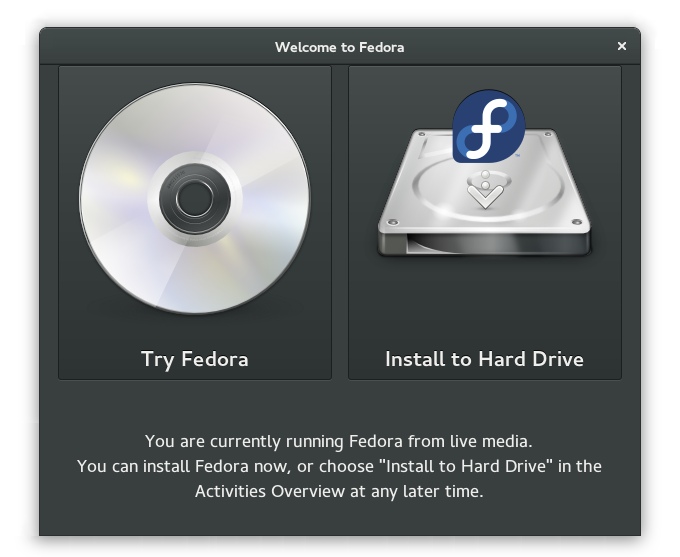
\includegraphics[width=.75\textwidth]{img/instalator-a}
\captionbelow{Nabootované instalační médium Fedory} \label{fig:instalator-a}
\end{center}
\end{figure}

Pro poslední dva body platí zásadní věc. Musíme si pečlivě ověřit, na který disk provádíme zápis instalačního ISO obrazu. Provádíme-li to na \emph{MS~Windows}, musíme ctít název diskového oddílu přiřazenému flashdisku, kam chceme zápis provést (nejčastěji \texttt{D:} či \texttt{E:}). Pod Linuxem pak musíme ověřit totéž (flashdisk bude typicky \uv{\texttt{/dev/sdX}}, kde \texttt{X} bude specifické písmeno). Asi nejlepší a nejbezpečnější cesta, jak toto zjistit, je použít aplikaci \emph{Disky}, která zobrazuje mnoho detailních informací a daném zařízení.

\section*{Instalace Fedory}
\begin{enumerate}

\item\emph{Bootování} -- \sloppy{ať už jsme si vytvořili jakékoliv bootovatelné médium, musíme se ujistit, že máme v~BIOSu na počítači, kde instalaci provádíme, nastavenou korektní bootovací sekvenci. Na prvním místě musí být zařízení, kde je zapsaný instalační obraz systému. Do BIOSu se dostaneme při spuštění počítače stiskem klávesy, která závisí na výrobci zařízení\linebreak{(typicky~\keystroke{Delete},} {\keystroke{F1},} {či~\keystroke{F2}).}} Často je také možné zvolit bootovací zařízení zcela bez vstupu do~BIOSu stiskem klávesy \keystroke{F12}.

\begin{figure}[t]
\begin{center}
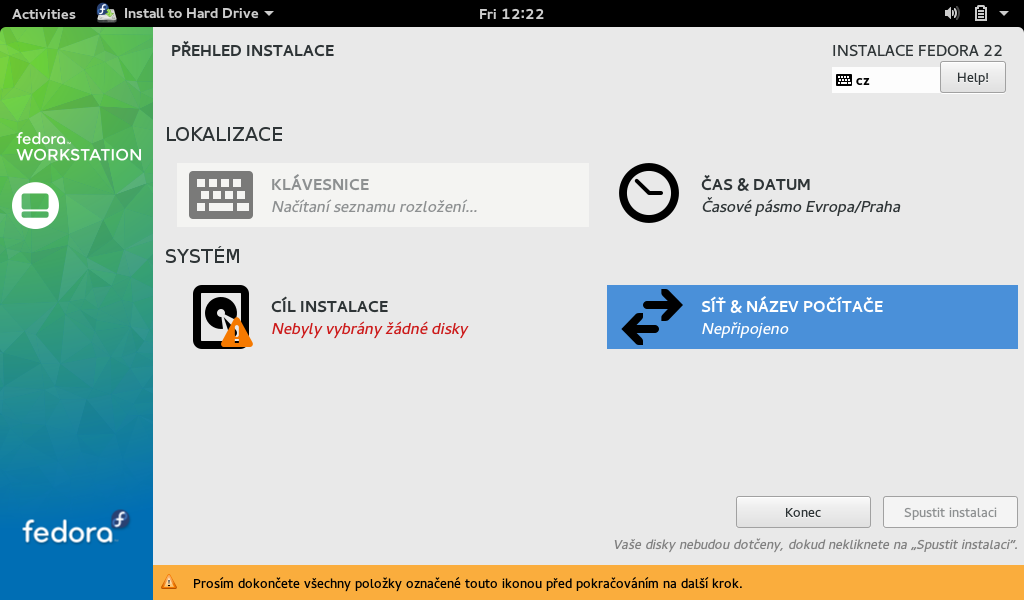
\includegraphics[width=\textwidth]{img/instalator-b}
\captionbelow{Instalátor Fedory} \label{fig:instalator-b}
\end{center}
\end{figure}

\item\emph{Úvodní obrazovka} -- po úspěšném nabootování uvidíme úvodní obrazovku, kde můžeme volit primárně mezi samotnou instalaci Fedory (a bootování do živého obrazu), nebo ověřením instalačního média. Zvolíme-li instalaci, budeme zanedlouho postaveni před volbu, jestli si chceme systém vyzkoušet, nebo nainstalovat na pevný disk. První volba není fatální, Fedoru můžeme zkoušet libovolně dlouho a k~instalaci se kdykoliv vrátit přes ikonu v~menu.

\pagebreak

\item\emph{GNOME Shell} -- pokud jsme zvolili možnost vyzkoušet, uvidíme před sebou tzv. prostředí \emph{GNOME~Shell}, které je typické nahoře umístěným výrazným panelem se základními ovládacími prvky. Vlevo nahoře je klíčové tlačítko činnosti, přes které se lze dostat k~nainstalovaným aplikacím (a zmíněné možnosti instalovat systém), vpravo naopak menu relevantní zejména pro nastavení sítě a možnosti restartu či vypnutí systému.

\item\emph{Instalátor} -- když zvolíme možnost instalovat na pevný disk, jsme postupně provázeni pomocí přehledného průvodce. Volíme krok za krokem jazyková nastavení, časové pásmo, až se dostaneme k~bodu rozdělení disku. Čili k~zásadnímu bodu řešícímu, kam se Fedora fyzicky nainstaluje. Fedora nabízí automatické rozložení, při kterém oddíly vytvoří sama, a samozřejmě i rozdělení ruční. Je také možné nastavit, které oddíly budou šifrované.

\item\emph{Pevný disk} -- Fedora v~této fázi umožňuje i vytvoření tzv. dualbootu, čili provozování dvou operačních systémů v~rámci jednoho počítače. Není problém ji tak doinstalovat vedle už existující instalace \emph{MS~Windows}. V~rámci dialogu je vlevo po celou dobu k~dispozici přehled existujících oddílů. Než změny potvrdíte, pečlivě si zkontrolujte, že jsou tam všechny (např. oddíly jiných operačních systému), které tam mají být. Po odsouhlasení tohoto kroku proběhnou nevratné změny a zápis nového rozložení na disk.

\item\emph{Závěr} -- zatímco se systém instaluje, vyplníme několik zásadních údajů, jako je heslo roota (administrátora) a vytvoříme uživatelský účet, pod kterým budeme běžně pracovat (a opět mu nastavíme heslo). Pozor, Fedora uplatňuje, na rozdíl od mnoha dalších linuxových distribucí, klasický přístup k~uživatelským účtům, při kterém účet uživatele root není zakázaný. Potřebujeme tedy nastavit a znát minimálně dvě hesla. Nevyhovuje vám toto nastavení? Nevadí, i u~našeho běžného účtu můžeme zaškrtnout volbu \uv{Správce}, která nám umožní velkou část správcovské činnosti stvrdit i pod naším běžným účtem a tedy i jeho heslem.

\item\emph{A~je hotovo} -- celá instalace by neměla zabrat více než několik desítek minut. Po restartu a přihlášení provedeme ještě několik krátkých poinstalačních nastavení (a pokud jsme měnili nastavení bootování, uvedeme ho do původního stavu) a systém je připraven. Zdařilo se? Můžeme tak začít používat Fedoru v~celé její kráse!
\end{enumerate}

\chapter*{První kroky v~systému}

\section*{Rozkoukáváme se}
Máme před sebou prostředí GNOME Shell. Klíčovým místem pro nás je už zmíněný levý horní roh (tlačítko \emph{Činnosti}), přes který se dostaneme k~vlevo umístěnému menu s~oblíbenými aplikacemi. Stačí do něj najet myší (nebo stisknout levou klávesu \uv{Super}, \uv{Start}, \uv{Meta}, nebo jak ji sami znáte). Jak se dostat ke všem aplikacím? V~menu nalezneme zcela dole ikonu se sadou čtverců \emph{Zobrazit aplikace}. Klikneme na ni a nyní máme aplikace přehledně vyskládané před sebou. Prostředí je velmi intuitivní. Znáte název aplikace? Nebo jen pár prvních písmen? Pak stačí začít psát (nebo použít vyhledávací pole zcela nahoře). Vyhledávání ale neprobíhá pouze mezi aplikacemi, hledá se i mezi kontakty, soubory, možnostmi nastavení a dalšími prvky.

\section*{Pojďme o~něco hlouběji}
Na co se dále zaměřit při běžné práci v~\emph{GNOME}? Předně si všimněte, že okna mají pouze tlačítko pro zavření. Proč je tomu tak, si vysvětlíme při popisu dalšího režimu, minimalizace v~prostředí \emph{GNOME} totiž postrádá smysl a maximalizovat okno lze tažením k~horní hraně obrazovky nebo poklikáním na lištu okna. Úkolem prostředí v~tomto režimu je co nejméně překážet, proto je zobrazen pouze horní panel. Na následujícím obrázku si vysvětlíme hlavní prvky tohoto režimu.

\begin{figure}[t]
\begin{center}
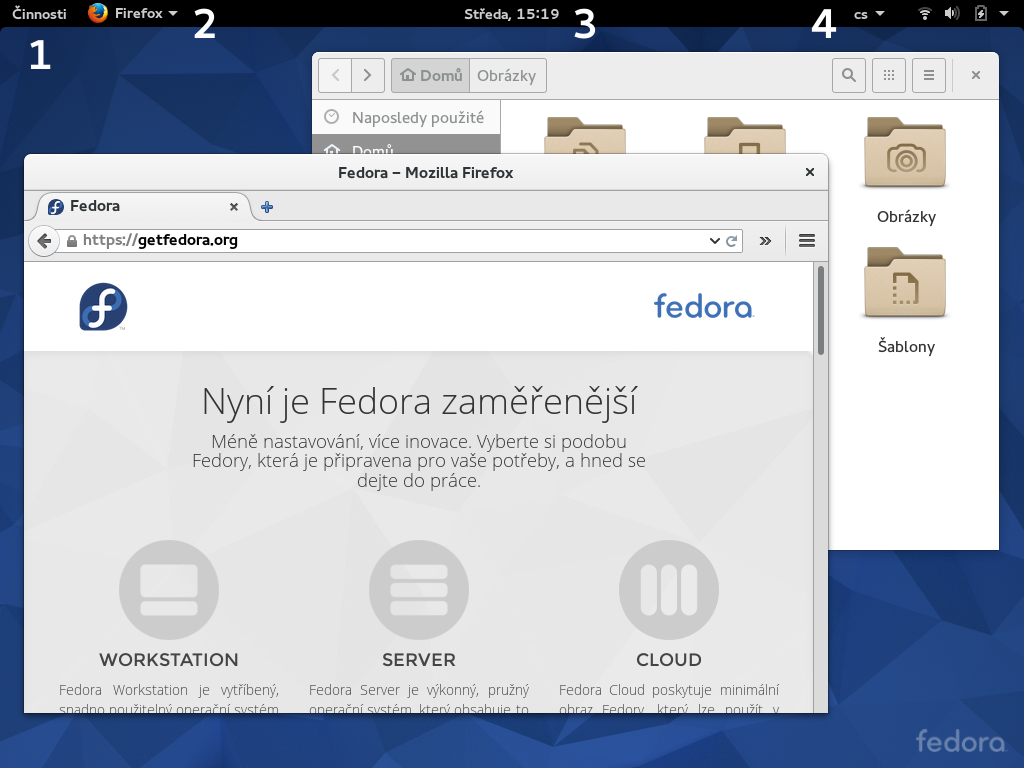
\includegraphics[width=\textwidth]{img/shell-a}
\captionbelow{shell-a.} \label{fig:shell-a}
\end{center}
\end{figure}

\begin{enumerate}
\item\emph{Činnosti} -- jde o~už výše zmíněný prvek, který slouží pro přepnutí do režimu \emph{Činnosti}, jenž je detailněji popsán níže. Je to výchozí bod, přes který se dostaneme k~většině úkonů, které chceme v~systému provádět.

\begin{figure}[t]
\begin{center}
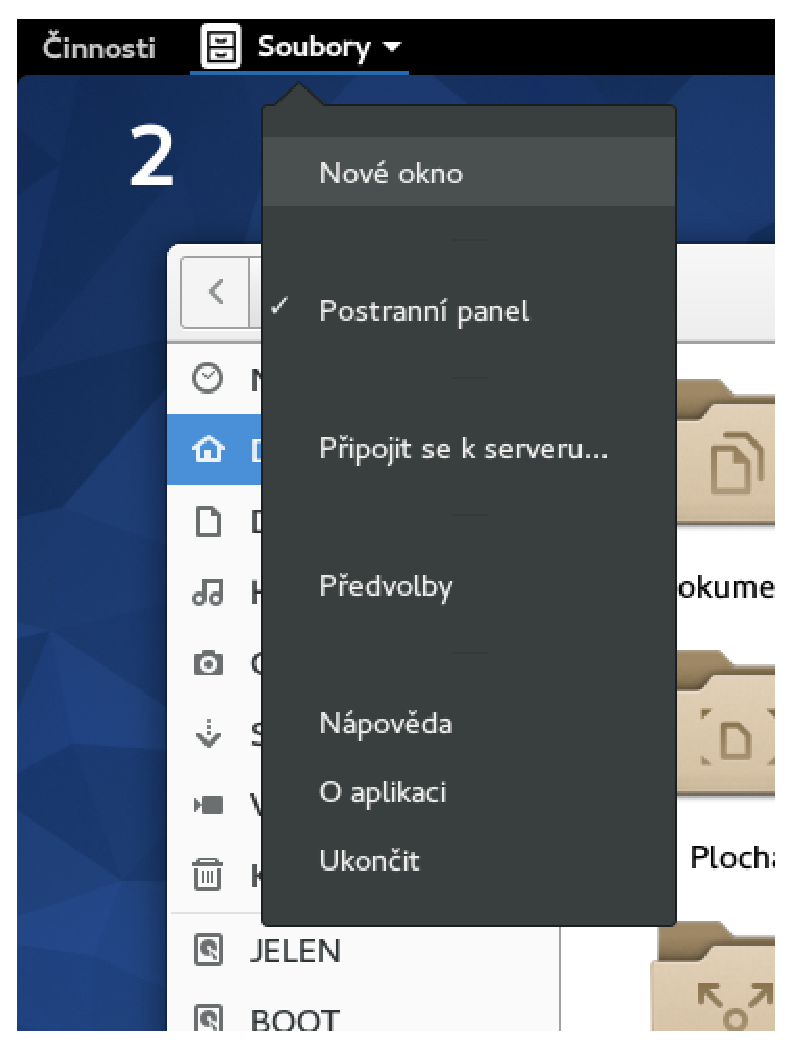
\includegraphics[width=\textwidth]{img/menu-aplikace}
\captionbelow{menu-aplikace.} \label{fig:menu-aplikace}
\end{center}
\end{figure}

\item\emph{Nabídka aplikace} -- pod ikonou momentálně aktivní aplikace naleznete nabídku, která se týká aplikace jako celku (nastavení aplikace, o~aplikaci apod.). Nabídky, které se týkají jednotlivých oken, se nalézají přímo v~okně aplikace. Ne každá aplikace tuto nabídku má. Pokud ji nemá, naleznete pod tímto tlačítkem pouze volbu \emph{Ukončit}.


\begin{figure}[t]
\begin{center}
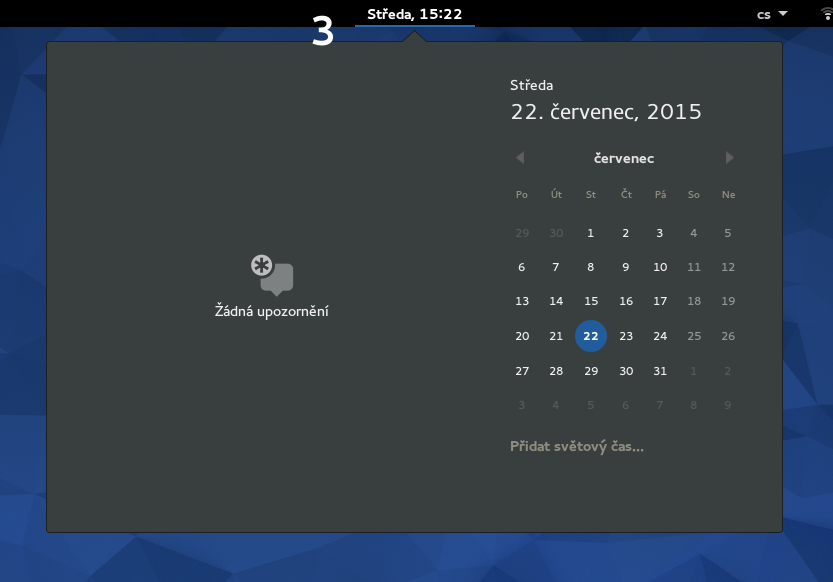
\includegraphics[width=\textwidth]{img/kalendar}
\captionbelow{kalendar.} \label{fig:kalendar}
\end{center}
\end{figure}


\item\emph{Hodiny a kalendář} -- pod zobrazením aktuálního dne a času naleznete kalendář a zmeškaná upozornění. Pokud využíváte jednu z~aplikací, které využívají kalendářový backend \emph{GNOME} (např. \emph{Evolution}), zobrazí se zde i události, které jste v~těchto aplikacích do kalendáře dříve uložili.

\begin{figure}[t]
\begin{center}
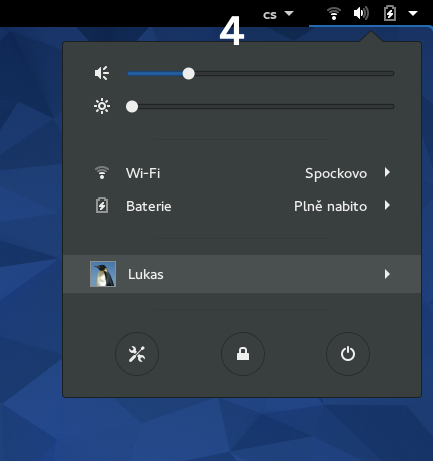
\includegraphics[width=\textwidth]{img/menu}
\captionbelow{menu.} \label{fig:menu}
\end{center}
\end{figure}

\item\emph{Nabídka uživatele} -- v~pravém horním rohu jsou k~dispozici nejdůležitější indikátory (připojení, zvuk, baterie atd.). Po kliknutí na ně se zobrazí nabídka, v~níž můžete nastavit hlasitost, úroveň jasu, připojení k~internetu, bluetooth a další věci. Třetí část nabídky obsahuje vaše jméno s~možnostmi odhlášení se nebo přepnutí do jiného uživatelského účtu. Zcela dole naleznete tři ikony. Ikona nalevo spouští nastavení systému, ta prostřední zamyká obrazovku a ikona napravo vám nabídne restartování nebo vypnutí systému.
\end{enumerate}

\begin{figure}[t]
\begin{center}
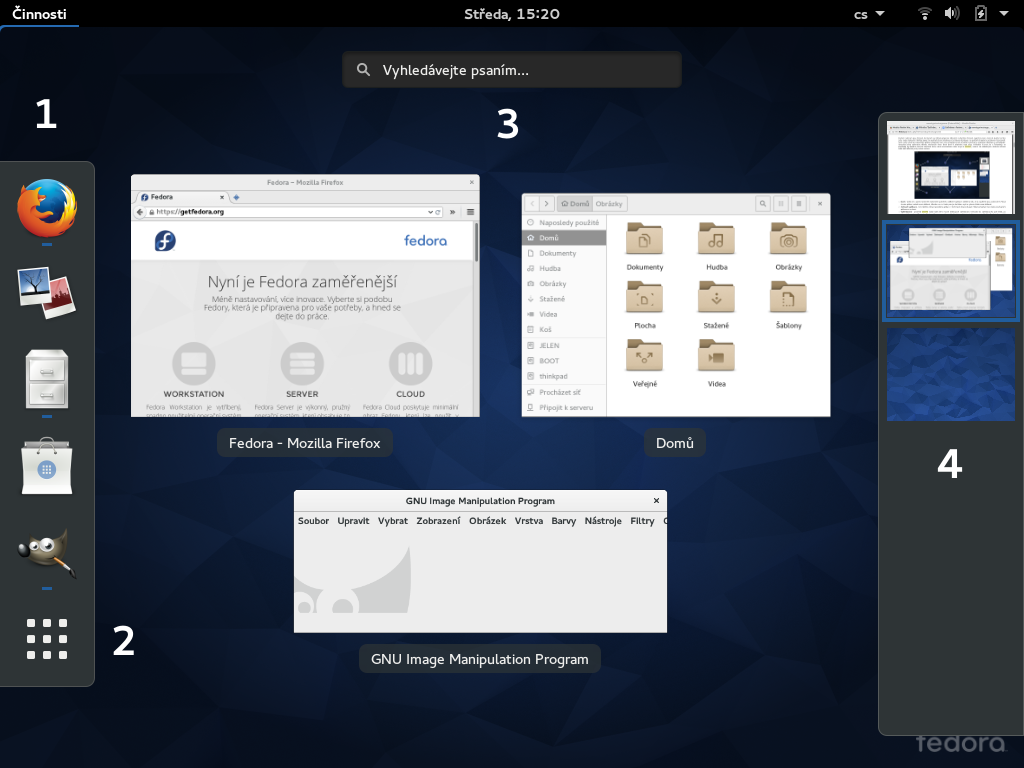
\includegraphics[width=\textwidth]{img/shell-b}
\captionbelow{shell-b.} \label{fig:shell-b}
\end{center}
\end{figure}

\section*{K~čemu slouží \emph{Činnosti}?}
Tento režim je určen pro spouštění aplikací, přepínání mezi nimi, přepínání mezi virtuálními plochami, organizaci desktopu a vyhledávání. Uprostřed obrazovky naleznete náhledy otevřených oken, které slouží k~přepínání mezi aplikacemi. Vzhledem k~tomu, že v~\emph{Činnostech} se poskládají do dlaždice všechna otevřená okna, nemá minimalizace oken smysl a, jak již bylo zmíněno, \emph{GNOME} ji nezná. Na následujícím obrázku můžete vidět další důležité prvky tohoto režimu

\begin{figure}[t]
\begin{center}
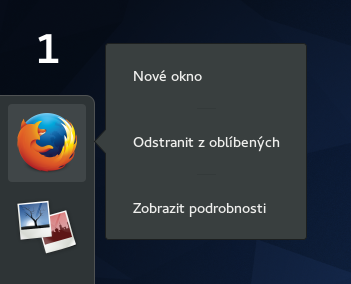
\includegraphics[width=\textwidth]{img/dash-b}
\captionbelow{dash-b.} \label{fig:dash-b}
\end{center}
\end{figure}

\begin{enumerate}
\item \emph{Dash} -- jedná se o~panel (\uv{menu}), na kterém naleznete spuštěné a oblíbené aplikace. Odlišíte je tak, že ty spuštěné jsou výrazně podtržené. Pokud chcete aplikaci zařadit mezi oblíbené, klikněte na ni v~Dashi pravým tlačítkem myši a vyberte \emph{Přidat mezi oblíbené}.

\begin{figure}[t]
\begin{center}

\includegraphics[width=\textwidth]{img/dash-a}
\captionbelow{dash-a.} \label{fig:dash-a}
\end{center}
\end{figure}

\item \emph{Zobrazit aplikace} -- opět již zmíněný prvek. Toto tlačítko zobrazí spouštěče aplikací. V~dolní části obrazovky pak můžete přepínat mezi často používanými aplikacemi a všemi aplikacemi.

\begin{figure}[t]
\begin{center}
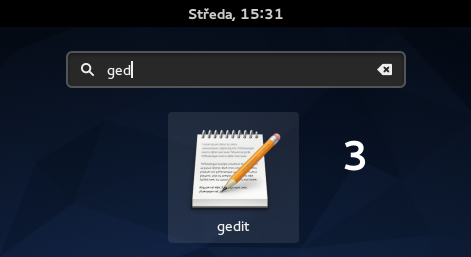
\includegraphics[width=\textwidth]{img/vyhledavani}
\captionbelow{vyhledavani.} \label{fig:vyhledavani}
\end{center}
\end{figure}

\item \emph{Vyhledávání} -- prostředí \emph{GNOME} nabízí také velmi mocné desktopové vyhledávání. Nemusíte do vyhledávacího pole klikat, po přepnutí do režimu \emph{Činnosti} můžete začít rovnou psát a vyhledávání se aktivuje. Jedná se o~nejrychlejší způsob, jak spouštět aplikace. Kromě nich ale můžete vyhledávat také dokumenty, obrázky, virtuální stroje, aplikace k~instalaci, kontakty, atd. Nebo také provádět jednoduché výpočty. Co se má v~\emph{Činnostech} vyhledávat, můžete nastavit v~systémových nastaveních pod položkou \emph{Hledání}.

\item \emph{Virtuální plochy} -- na levé straně můžeme najít náhledy virtuálních ploch, kterých lze mít více, aniž by bylo nutné mít více monitorů. Slouží k~organizaci oken a aplikací. \emph{GNOME} nemá fixní počet ploch. Naopak, jejich počet je dynamický. Je jich vždycky tolik, na kolika z~nich máte aktuálně umístěná okna, a jednu prázdnou navíc, která je připravená k~použití. Když na ni přetáhnete okno, vytvoří se další prázdná a naopak. Přetahovat okna mezi plochami můžete přímo v~náhledech, případně můžete přetáhnout náhled ze středu obrazovky do jednoho z~náhledů. Přepínat mezi virtuálními plochami můžete také přímo v~pracovním režimu pomocí klávesové zkratky $\keystroke{Ctrl}+\keystroke{Alt}+\keystroke{šipka $\uparrow$}\,/\,\keystroke{šipka $\downarrow$}$.

\item \emph{Náhledy otevřených oken} -- slouží k~přehledu o~tom, jaká okna máte otevřená, a také k~přepínání mezi nimi. Přepnutí do vybraného okna provedete najetím myši na okno a kliknutím. Mezi okny můžete přepínat také klávesami. Stačí po přepnutí do \emph{Činností} stisknout klávesu $\keystroke{šipka $\downarrow$}$ a potom pomocí šipek navigovat mezi okny. Přepnutí do vybraného okna provedete klávesou $\keystroke{Enter}$.
\end{enumerate}

\section*{Základní nastavení}
\emph{Uživatelská a systémová nastavení} Fedory nalezneme tak, že stejně jako u~dříve popsaného způsobu napíšeme slovo \uv{nastavení}, nebo přes samopopisnou ikonu v~menu na liště zcela vpravo nahoře. Nastavení jsou členěna do přehledných kategorií (\emph{Osobní}, \emph{Hardware} a \emph{Systém}), kde je možné konfigurovat vše od uživatelských účtů, přes pozadí plochy, až po tiskárny. Naprostá většina běžné konfigurace bude probíhat právě zde. Aplikace umožňuje i propojení s~množstvím online účtů, tedy s~cloudovými službami, ať už používáte ownCloud, Google, Facebook a další. Takto přidaný účet umožní přístup k~službám a datům daného poskytovatele a ostatním aplikacím. Používáte online chat? Potřebujete kontakty? Nic už není nutné zadávat znovu.


\begin{figure}[t]
\begin{center}
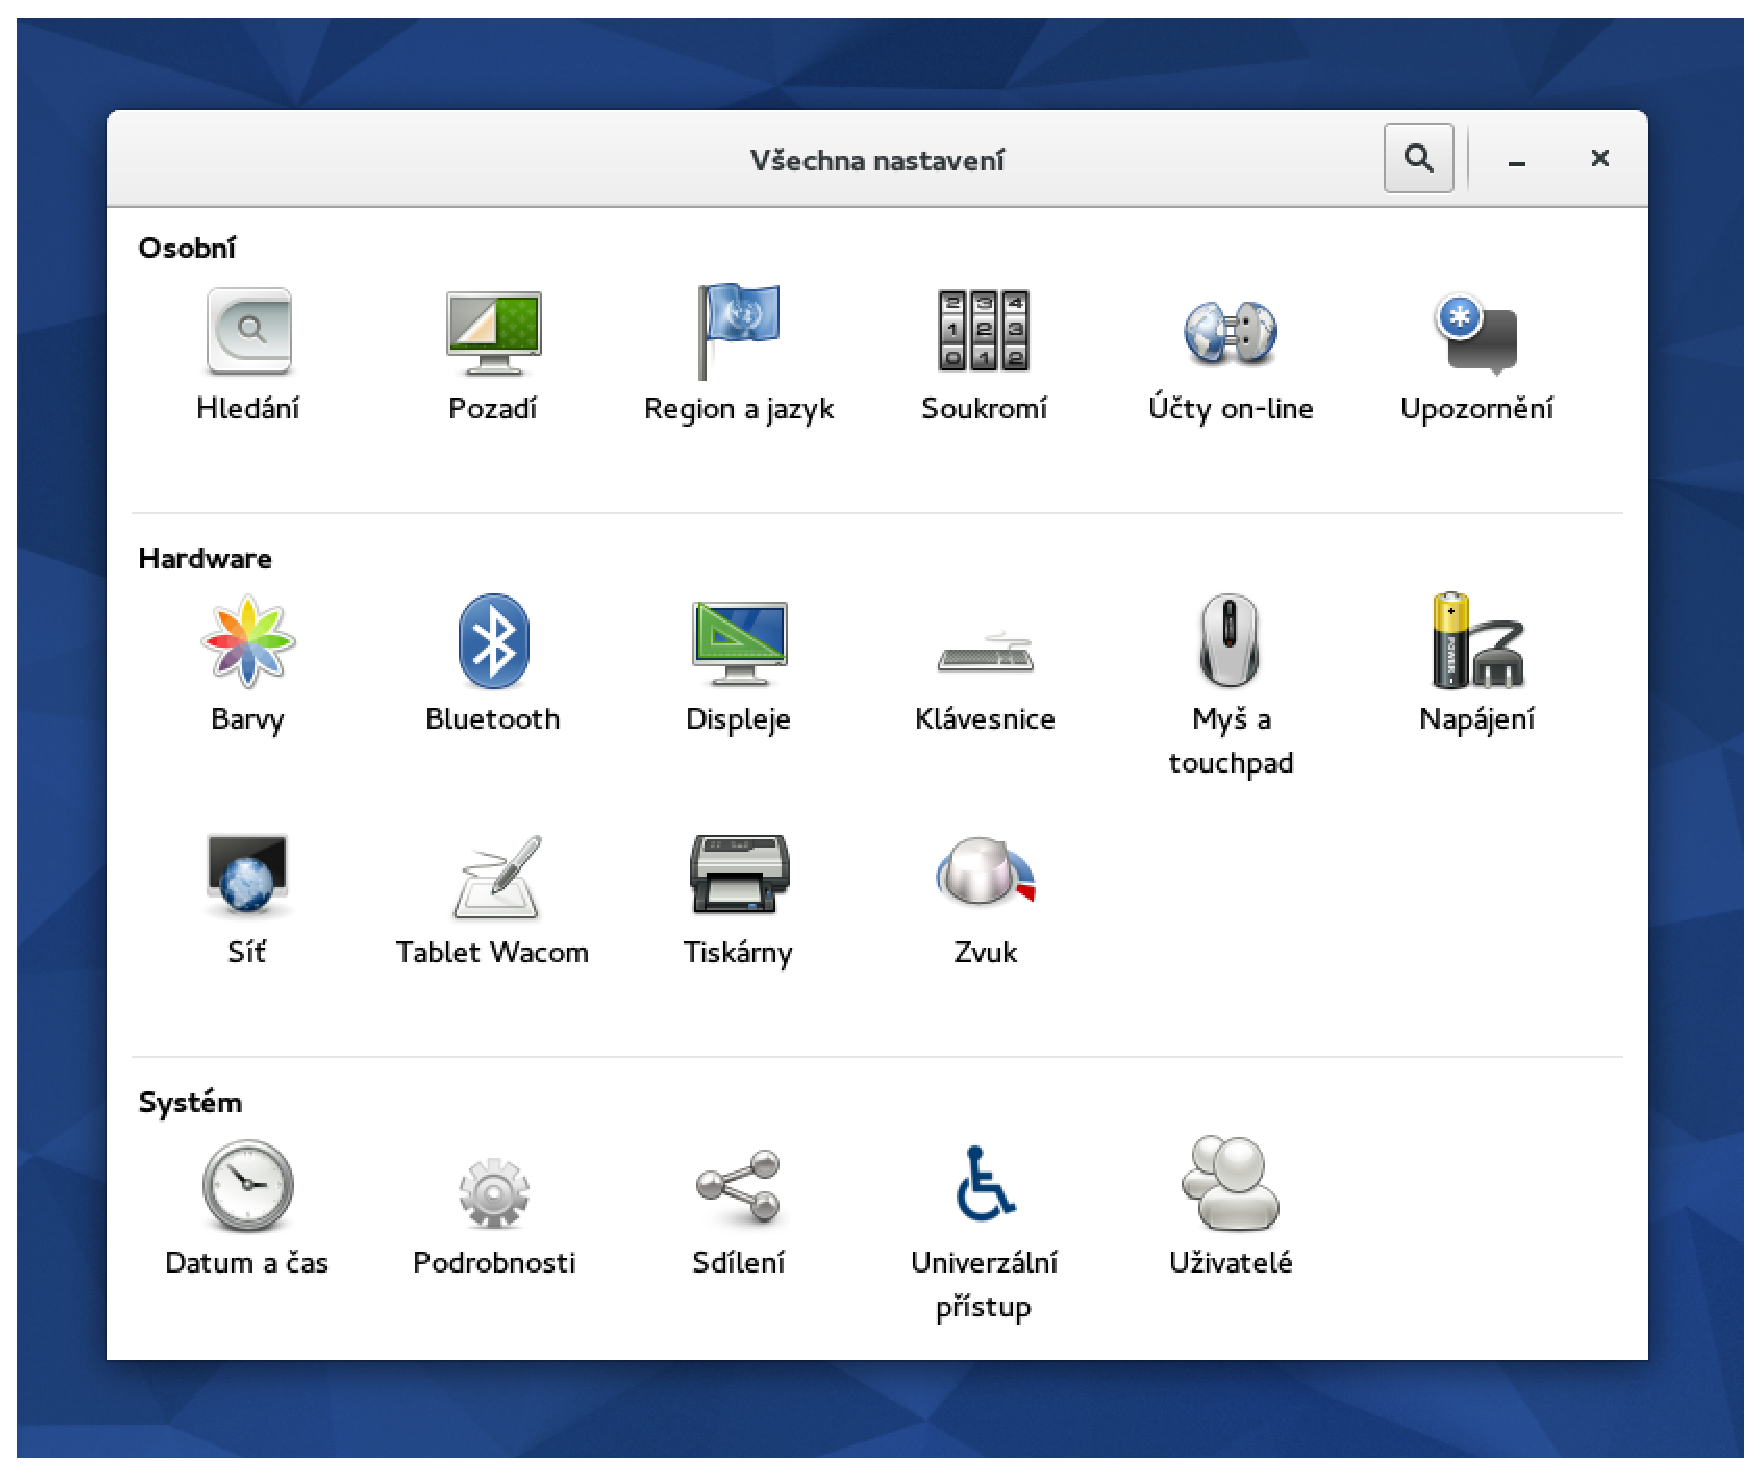
\includegraphics[width=\textwidth]{img/nastaveni}
\captionbelow{nastaveni.} \label{fig:nastaveni}
\end{center}
\end{figure}

\section*{Instalace nového software}
Fedora už v~základu obsahuje mnoho potřebných aplikací (webový prohlížeč \emph{Mozilla~Firefox}, kancelářský balík \emph{LibreOffice}, multimediální přehrávač \emph{Totem} a desítky dalších). Co když ale potřebujeme více programů? Ne všechen software může být zahrnut do výchozí instalace systému, je ale dostupný v~tzv. repozitářích, z~nichž lze daný program jednoduše stáhnout. Repozitář je tvořen sadou serverů a jejich zrcadel, kde jsou umístěny balíky s~různými aplikacemi a knihovnami. Slyšeli jste o~\uv{appstore} na různých mobilních platformách? Pak jste velice blízko, základní princip je stejný. Chcete nějaký program stáhnout z~webu a nainstalovat? Zkuste se nejprve podívat, zda není k~dispozici v~repozitářích. Na Linuxu se tak instaluje naprostá většina aplikací. Jak tedy na to?

\begin{enumerate}
\item \emph{Grafický správce} -- aplikace \emph{Software} je přesně ten druh programu, který znáte z~libovolné mobilní platformy. Je to elegantní a přehledná vstupní brána do repozitářů, kde lze dle názvu (nebo v~rámci kategorie) vyhledávat celistvé aplikace a různé doplňky pro systém. Každá aplikace zde má svůj přehledný popis včetně licence a své velikosti. Stále platí: vše je opensource, vše je bezplatné. Přes nástroj \emph{Software} můžeme aplikace samozřejmě i odinstalovat a setkáme se s~ním vždy, když budeme systém (a balíky v~něm) aktualizovat.

\begin{figure}[t]
\begin{center}
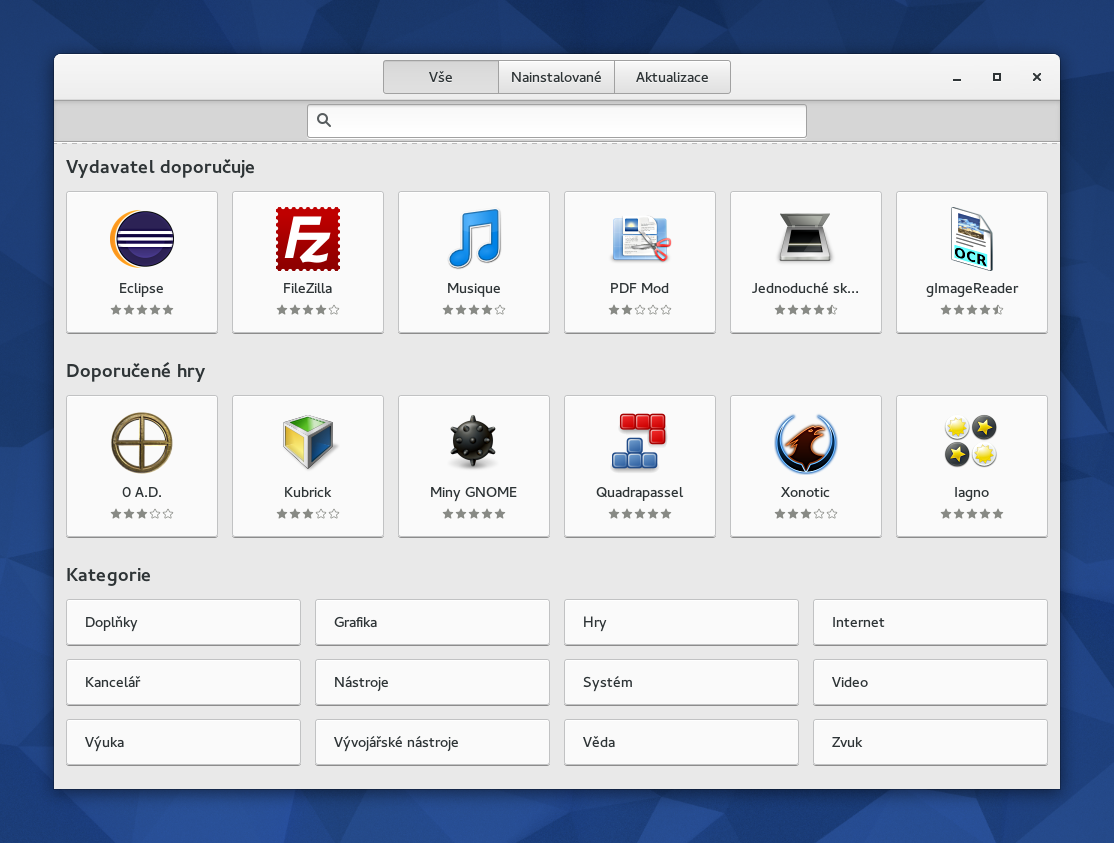
\includegraphics[width=\textwidth]{img/software}
\captionbelow{software.} \label{fig:software}
\end{center}
\end{figure}

\item \emph{Nástroj DNF} -- skrze nástroj \emph{Software} lze v~repozitářích dohledat hlavně ucelené spustitelné aplikace. Není ale určen na dohledání jednotlivé (třeba vývojářské) knihovny, dokumentace nebo různých dílčích utilit. Ve Fedoře je přitom takřka dvacet tisíc balíků, zdaleka ne všechny však obsahují pouze aplikace. Pro přístup ke všem balíkům (a jejich vyhledávání, instalaci, apod.) můžeme použít nástroj \emph{dnf} (určený pro práci v~shellu, není však těžké se jej naučit užívat) nebo jeho nadstavbu \emph{Yum extender (DNF)}, která je opět grafická a dává nám veškerý uživatelský komfort.
\end{enumerate}

\section*{Kodeky a další software}
Co když nějaký software k~dispozici v~repozitářích není? I~taková situace může nastat. Často se jedná o~specifický kodek nebo ovladač. Takový software nemusí být nezbytně placený, může být volně dostupný, ale už ho není (z~licenčních, nebo patentových důvodů) možné zahrnout do Fedory. Tady nastupují repozitáře třetích stran, které nejsou spravované ani jinak spojené s~Fedorou, ale mohou být velmi užitečné. (Dodejme, že za tyto zdroje softwaru nenese Fedora Project zodpovědnost a že nemusí mít vyřešenou právní nezávadnost podle autorského a patentového práva.)

\begin{enumerate}
\item \emph{Firemní repozitáře} -- korporace jako Google nebo Adobe nabízejí zdroje software obsahující jejich produkty. Jsou to různé vývojářské utility, ale i programy jako \emph{Google Chrome}, \emph{Adobe Flash plugin} a další. Jak jednou z~jejich webu nainstalujeme balík přidávající do našeho systému repozitář, vidíme dostupný software v~nástrojích stejně tak jako dříve zmíněný \emph{Software} nebo \emph{dnf}. Obdobným způsobem ho pak také spravujeme.

\item \emph{Další repozitáře} -- existují velké zdroje software třetích stran s~množstvím balíků, ke kterým např. nemáme k~dispozici zdrojové kódy nebo jsou jinak nevyhovující, ale které jsou stále užitečné. Multimediální kodeky a různé specifické ovladače pak můžeme nalézt v~repozitářích jako je (asi nejznámější) \emph{RPMFusion}. Instalace balíků pak opět probíhá analogicky.

\item \emph{Copr repozitáře} -- na rozdíl od předchozích dvou zmíněných variant jsou repozitáře Copr za všech okolností licenčně čisté. Je snadné je přidat a jsou, vedle oficiálních repozitářů, momentálně největší zdroj softwaru pro Fedoru. Může se jednat o~nové verze desktopových prostředí, frameworků apod. Samozřejmě při práci s~nimi je vždy nutné zjistit, co přesně daný software v~systému způsobí. Naleznete je na adrese \url{copr.fedoraproject.org}.

\end{enumerate}

\chapter*{Jak Fedoru přizpůsobit?}

\section*{Rozšíření pro GNOME Shell}
GNOME Shell disponuje rozšířeními, jež jsou mocnou zbraní co do přizpůsobení systému jednotlivému uživateli. Instalují se přímo v~prostředí webového prohlížeče z~webu \url{extensions.gnome.org}. Jedná se o~stovky rozšíření, které doplňují nebo mění jednotlivé prvky uživatelského prostředí. Změny menu, ikon, panelů, indikace, zobrazení, přepínání oken a nesčetné množství dalších.

\section*{Vylaďovací nástroj GNOME}
Aneb \emph{GNOME Tweak Tool}. Nástroj zahrnutý ve Fedoře, pomocí něhož lze podrobně, až do nejmenších detailů, nastavit jemnosti, které výchozí konfigurační nástroj neobsahuje. Můžeme zde namátkou měnit znělku prostředí, přesné chování virtuálních ploch, chování při napájení, písma aplikací, klávesové zkratky a opět desítky dalších věcí. Ostatně, můžeme zde spravovat i výše zmíněná rozšíření.

%\begin{figure}[t]
%\begin{center}
%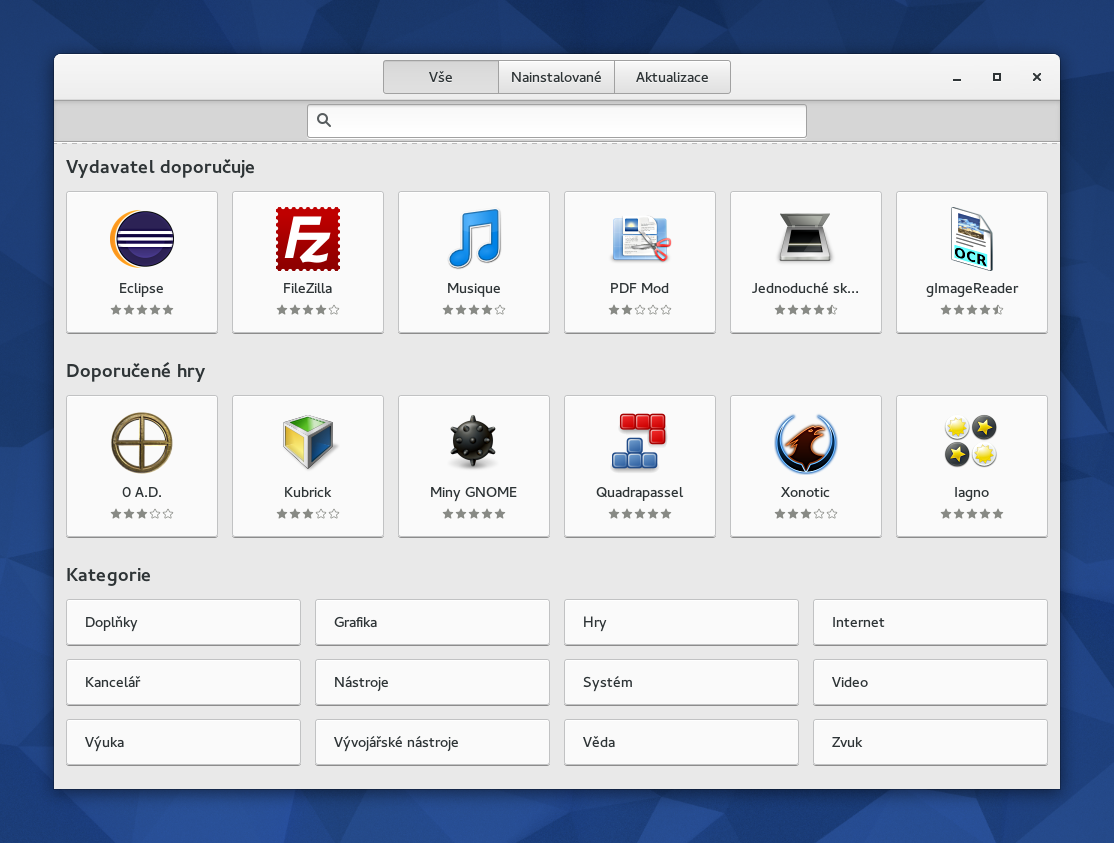
\includegraphics[width=\textwidth]{img/software}
%\captionbelow{GNOME Tweak Tool} \label{fig:software}
%\end{center}
%\end{figure}

\chapter*{Chcete vědět víc?}

\section*{Kam se podívat dál?}
Naše příručka má skromné ambice, ale co když narazíte na problém, který nejste schopni rychle vyřešit? Základní pravidlo zní: problém, který řešíte, už takřka jistě řešil někdo před vámi. Kam se tedy podívat?

\begin{itemize}
\item \url{fedora.cz} -- z~českých webů ve vztahu k~Fedoře zásadní stránky (a univerální rozcestník). Obsahuje množství článků, tipů a dalších informací.
\item \url{wiki.fedora.cz} -- příručka o~Fedoře, na které mnoho lidí odvedlo obrovské množství práce. Mnoho návodů, které hledáte, budou právě zde.
\item \url{forum.fedora.cz} -- fórum v~českém jazyce hodící se vždy, když nejste schopni problém vyřešit sami nebo když sami chcete nabídnout svou pomoc.
\item \url{fedoraforum.org} -- fórum v~anglickém jazyce s~rozsáhlou uživatelskou základou a dlouhou historií řešených problémů. Nyní už byste mohli být v~cíli.
\item \url{fedoramagazine.org} -- články o~dění kolem Fedory. Nové aplikace a oznámení.
\end{itemize}

\section*{Co když narazím na chybu?}
Je docela možné, že se dostanete do situace, kdy narazíte na chybu zcela novou. Co pak? Fedora používá bugzillu společnosti Red Hat, která je dostupná z~adresy \url{bugzilla.redhat.com}. (Nutno podotknout, že nezbytností při hlášení chyb je angličtina, alespoň na základní úrovni.) Není to ale jediná možnost, jak chybu ohlásit. Ve Fedoře je dostupný nástroj ABRT. Budeme-li citovat klasický snímek, pak daný nástroj vystihuje spojení \emph{\uv{každý přispívá podle svých možností}} a ABRT koná přesně v~tom duchu.

\section*{Další edice Fedory}
Zde se dostáváme k~věcem, ve kterých se Fedora odlišuje od obecného spektra linuxových operačních systémů. Fedora doznala své podoby ve třech hlavních edicích. Už dříve popsaná je edice \emph{Workstation}, dále pak tu máme edice \emph{Server} a \emph{Cloud}. Pojďme na ně. U~edice \emph{Server} lze vyzdvihnout aplikace jako Cockpit sloužící pro vzdálenou správu běžících serverů prostřednictvím webového prohlížeče nebo administraci serverových rolí přes Rolekit. U~edice \emph{Cloud} pak máme k~dispozici minimalistickou verzi Fedory, která umožňuje akorát nasazení kontejnerů. A~že existuje hned několik obrazů Fedory Cloud připravených pro nasazení v~prostředí \emph{OpenStack}, \emph{VirtualBox} a dalších.

\section*{Fedora a spiny}
Vše, co dosud padlo ve vztahu k~Fedora \emph{Workstation}, se týkalo výchozího cílení toho operačního systému, jehož desktopovým prostředím je \emph{GNOME~3} a jeho \emph{GNOME Shell}. Co když se ale chceme rozhlédnout dále? Ve Fedoře existují tzv. spiny, čili připravené instalační obrazy se specifickým cílením. Jste zvyklí na \emph{KDE Plasma}? Je tu \emph{KDE Plasma Desktop}. \emph{Xfce}? \emph{LXDE}? Pro vše tu jsou připravené obrazy. Ale ani u~Fedora spinů se nemusíme zastavit. V~dnešní době je velmi aktuální procesorová architektura ARM (nejčastější mobilní platforma, platforma pro různé vývojové desky à la Banana Pi, BeagleBone, nebo v~případě Fedora Remixu i Raspberry Pi). Stejně jako některé další linuxové operační systémy i Fedora má pro tuto architekturu připravené řešení ve formě jak serverové verze, tak minimálního instalačního obrazu pro obecné použití.


\end{document}
\endiput
